% $Id: AllegProposal.tex,v 1.8 2000/07/05 21:02:12 culver Exp $
% AllegProposal.tex
% by A. Thall
% 13. Feb 2003
%
% Small edits and a few additions made by R. Roos
% 21 Jan 2007
% Most particularly, the "box" around the thesis statement has been removed,
% section titles have been modified. The section named "Prior work II" has
% been commented out. The \topmargin has been changed to -.5in and the
% change to \parindent has been commented out.
% The filename "nausicaa.eps" has been changed to simply "nausicaa" so that
% pdflatex can be used on the file (and a file named "nausicaa.pdf" has
% been created using the "epstopdf" command).
% Several subsections have been added to illustrate subsection usage.
% The word "comp" has been replaced by "project" or "thesis" throughout.
% Other small changes have been made.
%
% This document provides a sample Senior Project Proposal template for use
% by students in Allegheny's CS and Applied Computing programs.

\NeedsTeXFormat{LaTeX2e}
\documentclass[11pt]{article}

%The following is used by WinEdt to set up cross-referencing to the BibTeX files
%It is NOT commented out---the comment lets it be simply ignored by non-WinEdt LaTeX compilers

%GATHER{mybibtexDB.bib}

\usepackage{setspace}
\usepackage{amsmath}
\usepackage{amssymb}
\usepackage{epsfig}
\usepackage{fancybox}
\usepackage{listings}
\usepackage{algo}
\usepackage{url}
\usepackage{multirow}
\usepackage{tabls}
\usepackage{afterpage}
\usepackage{booktabs}
\usepackage{epsf}
\usepackage{amsmath}   
\usepackage{amsfonts}
\usepackage{amssymb}
\usepackage{amsbsy}
\usepackage{bm}
\usepackage{epsfig}
\usepackage{rotating}
\usepackage{setspace}
\usepackage{tabls}
\usepackage{hhline}
\usepackage{float}

\setlength{\textheight}{9in}
\setlength{\textwidth}{6in}
\setlength{\oddsidemargin}{.25in}
\setlength{\topmargin}{-.5in}  % changed from -.25 by RSR on 1/21/07
%\parindent .5in    % commented out by RSR 1/21/07

%%% MY COMMANDS %%%

\usepackage{graphicx}
\usepackage{tabls}
\usepackage{afterpage}
\usepackage{float}
\usepackage{color}
\usepackage{amsmath,amsthm,amssymb}
\usepackage{verbatim}
\usepackage[parfill]{parskip}
\usepackage{tikz}
\usepackage{subcaption}
\usepackage{soul}
\usepackage[labelfont=bf]{caption}
\usepackage[framemethod=tikz]{mdframed}
\usepackage{multirow}
 
\renewcommand{\thefootnote}{\fnsymbol{footnote}}
\renewcommand{\ss}{\ensuremath{\|s\|}}
\newcommand{\N}{\mathbb{N}}
\newcommand{\Z}{\mathbb{Z}}
\newcommand{\deriv}[2]{\frac{\mathrm{d} #1}{\mathrm{d} #2}}
\newcommand{\pderiv}[2]{\frac{\partial #1}{\partial #2}}
\newcommand{\bx}{\mathbf{X}}
\newcommand{\ba}{\mathbf{A}}
\newcommand{\by}{\mathbf{Y}}
\newcommand{\bj}{\mathbf{J}}
\newcommand{\bs}{\mathbf{s}}
\newcommand{\B}[1]{\ensuremath{\mathbf{#1}}}
\newcommand{\Dt}{\Delta t}
\renewcommand{\d}{\mathrm{d}}
\newcommand{\mom}[1]{\langle #1 \rangle}
\newcommand{\cur}[1]{\left\{ #1 \right\}}
\newcommand{\xl}{{x_{i-1/2}}}
\newcommand{\xr}{{x_{i+1/2}}}
\newcommand{\il}{{i-1/2}}
\newcommand{\ir}{{i+1/2}}
\newcommand{\jl}{{j-1/2}}
\newcommand{\jr}{{j+1/2}}
\newcommand{\FOM}{\ensuremath{\text{FOM}}}

\graphicspath{{figures/}}


%put words in the hyphenation statement if you want to enforce
%how LaTeX should break them (or not) at the end of a line.
%\hyphenation{repre-sen-tations problems exact linear}
\hyphenation{itself}

%%%%%
%% Commented out -- RSR, 1/21/07
%%%%%
% The following provides a box to surround the thesis statement
%\newenvironment{Thesis}%
%{\begin{Sbox}\begin{minipage}{.95\linewidth}}%
%{\end{minipage}\end{Sbox}\begin{center}\fbox{\TheSbox}\end{center}}

\title{A High-Order Low-Order Algorithm with Exponentially-Convergent Monte Carlo for Thermal Radiative Transfer Problems}
\author{Dissertation Proposal \\ Simon Bolding, Nuclear Engineering Department}

\begin{document}


\singlespace
\maketitle

\doublespace
% This sets section-numbering to only include Section and Subsection numbers
\setcounter{secnumdepth}{2}

\section{Overview}

This document describes dissertation research over a new Monte Carlo algorithm for solution of
thermal radiative
transfer problems. Herein, a brief description of thermal radiative transfer and the
model problem are given, followed by a discussion of the standard Monte Carlo
solution method and other related research.  An overview of the methodology and
results performed thus far are given in Sec.~\ref{sec:perf}. Then, the remaining topics for completing this dissertation research
are discussed in Sec.~\ref{sec:prop}.  Finally, Sec.~\ref{sec:summary} provides a specific outline of the remaining research to be
investigated and computational results to be generated.

\section{Introduction}

\subsection{Thermal radiative transfer background}

Thermal radiative transfer (TRT) physics describe the time-dependent energy distributions of a photon
radiation field and a high-temperature material.  The material and radiation exchange
energy through absorption and emission of photons by the material.  
Accurate modeling of TRT physics becomes relevant in the high-energy,
high-density physics regime. Typical computational applications of TRT include simulation of inertial confinement fusion and
astrophysics phenomena. 
 The transport of
photons through a material is characterized by particle position, direction, and
frequency.  The material energy distribution is described by the material internal
energy (often described by material temperature) as a function of position.  The
high-dimensional space results in a difficult, nonlinear transport problem.

 This research will focus on a simplified 1D slab-geometry and
 frequency-integrated (grey) TRT model.  The governing equations for this simplified model are the radiation and material
 energy balance equations
\begin{align}\label{ho_cont}
    \frac{1}{c}\pderiv{I(x,\mu,t)}{t} + \mu \pderiv{I(x,\mu,t)}{x} + \sigma_t
    I(x,\mu,t)
&= \frac{\sigma_s}{2} \phi(x,t) +\frac{1}{2} \sigma_a a c T^4(x,t)
    \\ \label{t_cont}
  \rho c_v \pderiv{T(x,t)}{t} &=  \sigma_a \phi(x,t) - \sigma_a a c T^4(x,t).
\end{align}
In the above equations the fundamental unknowns are the material temperature $T(x,t)$ and
the angular intensity $I(x,\mu,t)$ of radiation, where $x$ is the position, $t$ is the time, $\mu$ is
the $x$-direction cosine of the photon direction of travel, and $a$, $c$, $\rho$,
and
$c_v$ are the radiation constant, speed of light, material mass density, and material specific heat; $\sigma_a$, $\sigma_s$, and
$\sigma_t$ are the absorption, scattering, and total
cross sections (cm$^{-1}$), respectively.  The scalar radiation intensity $\phi(x,t)=\int_{-1}^1
I(x,\mu,t) \d \mu$ is related to the radiation energy density
$E$ (with typical units Jks cm$^{-3}$ sh$^{-1}$) by the relation $E = \phi/c$.   The equations are
strongly coupled through the gray Planckian emission source $\sigma_a a c T^4$, which
is a nonlinear function of temperature, and the radiation absorption
term $\sigma_a \phi$.  In general, the material properties are a function of $T$.  The temperature dependent material properties and
absorption and reemission physics lead to systems that require accurate modeling of
photon transport through a  mix of
streaming and optically-thick, diffusive regions.  Although in most physical
applications material motion is present, it is not the focus of this research and will not
be considered.  The purpose of the proposed research is to demonstrate the ability 
of a new algorithm to provide highly-accurate and efficient solutions to
Eq.~\eqref{ho_cont} and Eq.~\eqref{t_cont}.

\subsection{The implicit Monte Carlo method}

The Monte Carlo (MC) method~\cite{shultis_mc} is a standard computational method in
the field of radiation transport.
 The implicit Monte Carlo (IMC) method~\cite{fnc}
is the most common approach for applying the MC method to TRT problems. The IMC
method partially linearizes Eq.~\eqref{ho_cont} and Eq.~\eqref{t_cont} over a discrete time
step and lags material properties to produce a linear transport equation, which can be solved with MC
simulation.  The linear transport equation contains an approximate emission source
and effective scattering cross section that represent
absorption and reemission of photons over a time step.  The transport equation is
solved with MC simulation 
to advance the distribution of radiation to the end of the time step and determine
the energy absorbed by the material over the time step.  The energy absorption by
the material is tallied over a discrete spatial mesh, computed with cell-averaged
quantities.
  The energy absorption in each mesh cell is used to directly estimate
a new end of time step material temperature based on the linearized material
energy balance equation. Integration of the
time-variable is treated continuously over the time step via MC sampling, but the
linearized Planckian source in the transport equation is based on a time-discrete
approximation.
  

The IMC method has some limitations.  In optically thick regions, or for
large time steps, the
effective scattering dominates interactions.  In these diffusive regions IMC
becomes computationally expensive. Acceleration methods typically attempt to improve
efficiency by allowing particles to take discrete steps through optically-thick
regions based on a spatially-discretized diffusion approximation~\cite{imd,ddmc}. 
Another issue occurs due to the approximate linearization of the system which can not
be iteratively improved due
to the high computational cost of the MC transport.  For some problems, the
linearization can yield non-physical results that violate the discrete maximum
principle if the time step size is too large or the cell size is too
small~\cite{wollaber2013discrete}.  The violation of the maximum principle results in
the material temperature being artificially higher than the boundary conditions and
sources should physically allow.  The violation is caused by the temperature in the
emission source not being fully implicit in time due to the necessary linearization.
The work in~\cite{iimc_gentile} uses less-expensive MC iterations to produce an implicit system
which prevents this from happening, but has very slow iterative convergence in diffusive
problems.  
In IMC, temperature-dependent
material properties, in particular cross sections, are evaluated at the previous-time
step temperature. These lagged cross sections can produce inaccurate solutions but
do not cause stability issues.  

%PICTURE OF STANDARD MC SOLUTION AND MAXIMUM PRINCIPLE VIOLATION?

%WHAT IS UP WITH THE WEIRD DIFFUSION LIMIT

For TRT simulations, inaccurate spatial representation of the emission source over a cell can result in
energy propagating through the domain artificially fast, yielding non-physical
results referred to as ``teleportation error"~\cite{teleportation}.  The IMC method uses a fixup known as source tilting
to mitigate this problem.  Source tilting reconstructs a more accurate
linear-discontinuous representation of the
emission source within a cell based on the cell-averaged material temperatures in adjacent
cells. This linear reconstruction is also necessary to preserve the asymptotic equilibrium diffusion
limit (EDL), at least for a more general time step size and class of problems than for a piece-wise constant representation~\cite{diff_limit_imc}.  Preserving the equilibrium diffusion limit is an
important aspect of a numerical method for TRT problems. 
In this limit, cells are optically thick and diffusive, and the material
and radiation energy fields approach equilibrium.
Spatial discretizations which do not preserve the EDL can produce inaccurate
solutions, even though the mesh size should accurately capture the behavior of the solution~\cite{morel_newton}.

\subsection{Previous work on moment-based acceleration methods}

An alternative application of MC to the TRT equations is moment-based hybrid MC methods.
Recent work has focused on so-called high-order low-order (HOLO)
methods~\cite{willert,park,rmc,ans_2014}. These methods involve fixed-point
iterations between high-order (HO) MC solution of a transport equation and a deterministic LO
system.  The low-order (LO)
operator is based on angular moments of the transport equation, formulated over a fixed
spatial mesh.  Physics operators that are time consuming for MC
to resolve, e.g., absorption-reemission physics, are moved to the LO
system.  The reduced angular dimensionality of the system and Newton methods allow for non-linearities in the LO equations to be fully
resolved efficiently~\cite{willert,park}.  The high-order (HO) transport problem is defined by 
Eq.~\eqref{ho_cont}, with sources estimated from the previous LO solution.  
The high-order (HO) transport equation is solved via MC to produce a high-fidelity solution for
the angular intensity.  The MC estimate of the angular intensity is used to estimate
consistency terms,
present in the LO equations, that require the LO system to preserve the angular accuracy of the
MC solution.   
These consistency terms are present in all spatial-regions of the problem, requiring
statistical variance to be reduced sufficiently throughout the entire domain of the
problem. 

Another area of related research is the application of
residual Monte Carlo.  The goal of these methods is to solve an auxiliary transport
equation for the error in some estimate of the intensity.  The error is then added to the
estimate of the solution, which can produce an overall solution for the intensity that has
less statistical noise than solution of the original transport equation would produce.  In~\cite{rmc}, the MC simulation
solves for the change in intensity from the previous time step. This has the potential to limit statistical noise
significantly in regions where the solution is near equilibrium.
The work in~\cite{rmc} used residual MC as a HO solver for 1D grey problems. The
  residual MC demonstrated impressive reduction in statistical variance.
  However, a piecewise constant representation was used for the
space-angle representation of the intensity, which
does not preserve the EDL and can be inaccurate in angularly complex regions of the
problem.  Similar to RMC, a difference formulation has been applied to another algorithm known as the symbolic IMC method
(SIMC), for the case of 1D frequency-dependent problems~\cite{simc_const}.  SIMC forms a
standard FE solution to the material energy balance equation, and uses symbolic
weights in the MC transport to solve for expansion coefficents.  The difference
formulation modifies the transport equation to solve for unknowns representing the
deviation of the intensity from
equilibrium with the material energy.  The difference
formulation was also applied to a linear-discontinuous FE spatial
representation of the emission source, demonstrating accuracy in the EDL~\cite{simc}. 
Both~\cite{simc_const} and~\cite{rmc} produced minimal
statistical noise in slowly varying problems where the behavior of the system is near
equilibrium. 

\subsection{Proposed algorithm}

The research proposed herein provides a new HOLO algorithm for radiative transfer.
In this work, we propose an S$_2$-like LO operator~\cite{wolters}
in conjunction with an exponentially-convergent MC (ECMC) method~\cite{jake} for the
HO solver. Our LO system and approach to enforcing consistency contrast greatly from the typical formulation
in~\cite{rmc,willert,park}. We have derived the LO operator directly from the transport
equation, using a linear-discontinuous finite-element (LDFE) spatial
discretization.   
Exponentially-convergent Monte Carlo (ECMC)\cite{jake,ans_2014} provides an iterative algorithm that can efficiently
reduce statistical noise to acceptable levels with
significantly less particle histories than standard MC. In particular, ECMC is
exceptionally efficient in time-dependent TRT problems because information about the
intensity from the previous time step can be used as an accurate initial guess for
the new end of time step intensity.   However, implementation
of ECMC is non-trivial, requiring a finite-element representation of the solution in
all phase-space variables that are being sampled with MC.  
The method contains many of the desired qualities, such as
preserving the equilibrium diffusion limit, preserving the maximum principle, and in
particular, providing high-fidelity MC solution to the TRT equations in an efficient
manner.
%representation in the HO and LO systems enforces spatial consistency and ensures the
%solution correctly produce the equilibrium diffusion limit, a critical aspect
%for TRT equations.


\section{Performed Research}
\label{sec:perf}

\subsection{Overview of the HOLO Algorithm}

For simplicity, our HOLO method uses a backwards Euler discretization in time, as
well as constant specific heats and cell-wise constant cross sections. The time-discretized
equations are
\begin{align}
    \mu \pderiv{I^{n+1}}{x} + \left(\sigma_t^{n+1} + \frac{1}{c \Delta t }\right) I^{n+1}
&= \frac{\sigma_s}{2} \phi^{n+1} +\frac{1}{2} \left(\sigma_a a c T^4 \right)^{n+1} + \frac{I^n}{c \Delta t} \label{ho_trans} \\
\rho c_v \frac{T^{n+1} - T^n}{\Delta t} &= \sigma_a^{n+1} \phi^{n+1}
- \sigma_a a c (T^4)^{n+1} \label{lo_mat},
\end{align}
where $\Delta t$ is the uniform time step size, the superscript $n$ is used to indicate
the $n$-th time step. Cross sections are evaluated at the end of time step
temperature, i.e., $\sigma_a^{n+1}\equiv\sigma_a(T^{n+1})$.   

In the HOLO context, the LO solver models the physical scattering and
resolves the material temperature spatial distribution $T^{n+1}(x)$, for each time step.  The LO equations are formed via half-range 
angular and spatial moments of
Eq.~\eqref{ho_trans} and Eq.~\eqref{lo_mat}. The spatial moments are formed over a
finite-element
mesh and a linear-discontinuous spatial closure with upwinding is used to close the
system.  The angular treatment in the LO equations has the same form as those used in the
hybrid-S$_2$ method in~\cite{wolters},  with
consistency parameters that represent angularly-weighted averages of the intensity.
If the angular consistency parameters were estimated exactly, then
the LO equations preserve the exact angular-averaged solution,  neglecting spatial
discretization errors.  These consistency parameters are lagged in each LO solve,
estimated from the previous HO solution for the intensity, or from a previous time
step.  The discrete LO equations always conserve total energy, independent of the accuracy of the consistency terms.
It is noted that our LO operator is different from the nonlinear
diffusion acceleration (NDA) methods used by other HOLO methods~\cite{rmc,park,willert}.  In
NDA methods, an artificial term is added to the LO equations to enforce consistency and estimated using a
previous HO solution.  In our method we have simply algebraically 
manipulated space-angle moment equations to produce our consistency terms,
which will hopefully produce more
stability in optically-thick regions where NDA methods demonstrate stability issues.

The solution to the LO system is used to construct a LDFE spatial representation of
the scattering and emission sources on the right hand side of Eq.~\eqref{ho_trans}.
 This HO transport problem represents a characteristic method that uses MC to
invert the continuous streaming plus removal operator with an LDFE representation of
sources. We will solve this transport problem using ECMC~\cite{jake}.  The output from ECMC is
$\tilde{I}^{n+1}(x,\mu)$, a space-angle LDFE projection of the exact solution for
$I^{n+1}(x,\mu)$.  Once computed, $\tilde{I}^{n+1}(x,\mu)$ is used
to directly evaluate the necessary consistency parameters for the next LO solve.   The HO solution is not used to directly estimate a new
material temperature, which eliminates
typical operator splitting stability issues that require linearization of the
emission source in Eq.~\eqref{ho_cont}. 

The process of performing subsequential HO and LO solves, within a single time step, can be repeated to obtain an increasingly accurate solution for $\phi^{n+1}(x)$ and $T^{n+1}(x)$.  Thus, the HOLO algorithm, for the $n$-th time step, is
\begin{enumerate}
\item Perform a LO solve to produce an initial guess for $T^{n+1}(x)$
    and $\phi^{n+1}(x)$, based on consistency terms estimated with $\tilde{I}^{n}$.
\item Solve the HO system with ECMC for $\tilde{I}^{n+1}(x,\mu)$, based on the current
    LO estimate of emission and scattering sources.%$\sigma_s(T^k)\phi^{k}$ and $B(T)^{k}$.
\item Compute new LO consistency parameters with $\tilde{I}^{n+1}$.  
\item Solve the LO system with HO consistency parameters to produce a new
    estimate of $\phi^{n+1}$ and $T^{n+1}$.
\item Optionally repeat 2 -- 4 until desired convergence is achieved.
\item Store $\tilde{I}^{n}\leftarrow\tilde{I}^{n+1}$, and move to the next time step.
\end{enumerate}
The consistency terms force the HO
and LO solutions for $\phi^{n+1}(x)$ to be consistent to the order of the current HOLO
iteration error, as long as the LDFE spatial representation can accurately represent
$\phi(x)$ and $T(x)$.
%One HOLO fixed-point iteration $k$ denotes the process of an ECMC solve of the HO problem to estimate LO parameters, based on
%the current LO estimate of sources, followed by a solution of the 
%LO system for $T^{n+1}(x)$ and $\phi^{n+1}(x)$.


\subsection{The Low-Order Equations}

This section contain explicit details of the LO operator.
To form the LO system of equations, spatial moments are taken over each spatial cell $i$:
$x\in[x_{i-1/2},x_{i+1/2}]$, weighted with the standard linear finite element (FE)
interpolatory basis functions.  For example, the $L$  moment operator is defined by
\begin{equation}\label{x_mom}
\mom{\cdot}_{L,i} = \frac{2}{h_i} \int_{x_{i-1/2}}^{\xr} b_{L,i}(x) (\cdot) \d x,
\end{equation}
where $h_i=x_{i+1/2}-x_{i-1/2}$ is the width of the spatial element and
$b_{L,i}(x)=(x_{i+1/2}-x)/h_i$ is the FE basis function, for cell $i$, corresponding to position
$x_{i-1/2}$.  The right moment $\mom{\cdot}_{R,i}$ is defined with weight function $b_{R,i}(x)=(x -
x_{i-1/2})/h_i$. 
%It is noted in this notation $\mom{\phi}_{L,i}$ and
%$\mom{\phi}_{R,i}$ represent spatial moments of the intensity over cell $i$, opposed
%to $\phi_{L,i}$ and $\phi_{R,i}$, which represent the interior value of the linear
%representation of $\phi(x)$ at $x_\il$ and $x_\ir$ within the cell.
To reduce the angular dimensionality, positive and
negative half-range integrals of the angular intensity are taken.  The half-range
averages of $I$ are defined as $ \phi^+(x) = \int_0^{1} I(x,\mu) \d \mu$ and $ \phi^-(x) = \int_{-1}^{0} I(x,\mu) \d
\mu$, respectively.  Thus, in terms of half-range quantities, $\phi(x) = \phi^-(x) +
\phi ^+(x)$.  

Pairwise application of the $L$ and $R$ basis
moments with the $+$ and $-$ half-range integrals to Eq.~\eqref{ho_trans} 
ultimately yields four moment
equations per cell. As in~\cite{wolters}, algebraic manipulation is performed to form
intensity-weighted
averages of $\mu$, which we denote consistency terms.  
As an example, the equation resulting from application of the $L$ moment and
positive half-range integral is
\begin{multline}\label{lo_tran}
    -2{\mu}_{i-1/2}^{n+1,+} \phi_{i-1/2}^{n+1,+} + \cur {\mu}_{L,i}^{n+1,+}
  \mom{\phi}_{L,i}^{n+1,+}
  +  \cur\mu_{R,i}^{n+1,+}
  \mom{\phi}_{R,i}^{n+1,+} +  \left(\sigma_{t,i}^{n+1}+\frac{1}{c \Delta t} \right) h_i 
  \mom{\phi}_{L,i}^{n+1,+} \\-  \frac{\sigma_{s,i} h_i}{2} \left( \mom{\phi}_{L,i}^{n+1,+} +
  \mom\phi_{L,i}^{n+1,-}\right) = \frac{h_i}{2} \mom{\sigma_a^{n+1} a c T^{n+1,4}}_{L,i} +
  \frac{h_i}{c\Delta t}\mom{\phi}_{L,i}^{n,+},
\end{multline}
where the $\phi^+_{i-1/2}$ and $\mu^+_{i-1/2}$ terms represent face-averaged quantities at $x_{\il}$.  The negative direction and $R$ moment equations are
derived analogously.  The element-averaged angular consistency terms are defined in terms of half-range integrals, e.g.,
\begin{equation}\label{const}
    \cur{{\mu}}_{L,i}^{n+1,+} \equiv \frac{\mom{\mu I^{n+1}}_{L,i}^+}{\mom{I^{n+1}}_{L,i}^+} =  \frac{
{\displaystyle \frac{2}{h_i}} \int\limits_0^1 \int\limits_\xl^\xr \mu \, b_{L,i}(x)
I^{n+1}(x,\mu) \d x \d \mu } 
{{\displaystyle \frac{2}{h_i}} \int\limits_0^1 \int\limits_\xl^\xr \, b_{L,i}(x)
I^{n+1}(x,\mu) \d x \d \mu } .
\end{equation}
The $\mu_{i-1/2}^{n+1,+}$ term is defined analogously and represents an angular average on the face at $x_{\il}$.

To derive the LO material energy equations, $T(x)$ is represented spatially in
the LDFE trial space, i.e.,
$ T(x) \simeq T_{L,i} b_{L,i}(x) + T_{R,i} b_{R,i}(x),\quad x\in(x_{i-1/2},x_\ir)$.
Similarly, the emission term is represented in the material and radiation equations with the LDFE
interpolant $T^4(x)\simeq T_{L,i}^4 b_{L,i}(x) + T_{R,i}^4 b_{R,i}(x)$.   The $L$ and $R$ spatial moments are taken of the material
energy equation, using these definitions for $T(x)$ and $\sigma_a a c T^4(x)$ to simplify moments. For example, the final LO material energy
 equation resulting from application of the $L$ moment is
 \begin{multline}\label{lo_mat_dis}
     \frac{\rho_i c_{v,i}}{\Delta t}\left[ \left(\frac{2}{3}T_{L,i} + \frac{1}{3}T_{R,i}
        \right)^{n+1} - \left(\frac{2}{3}T_{L,i} + \frac{1}{3}T_{R,i}
    \right)^{n} \right]  + \sigma_{a,i}^{n+1} \left( \mom{\phi}_{L,i}^+ +
    \mom{\phi}_{L,i}^- \right)^{n+1} \\ = \sigma_{a,i}^{n+1}a c
\left( \frac{2}{3} T_{L,i}^4 + \frac{1}{3}T_{R,i}^4
        \right)^{n+1}.
\end{multline}
Cross sections have been assumed constant over each element, evaluated at the
average temperature within the element, i.e., $\sigma_{a,i}^{n+1} =
\sigma_{a,i}([T^{n+1}_{L,i}+T^{n+1}_{R,i}]/2)$.

\subsection{Closing the LO equations}

The six degrees of freedom (DOF) over each cell $i$ are the four moments $\mom{\phi}_{L,i}^+$,
$\mom{\phi}_{R,i}^+$, $\mom{\phi}_{L,i}^-$, and $\mom{\phi}_{R,i}^-$ and the two
spatial edge values $T_{L,i}$ and $T_{R,i}$. The relation between the volume and face averaged quantities and the angular consistency parameters (e.g., Eq.~\eqref{const}) are not known a priori. 
Currently, to close the LO system spatially, the standard LDFE approximation with upwinding is
used.  For example, for positive flow (e.g., Eq.~\eqref{lo_tran}) the face terms $\mu_{i-1/2}$ and $\phi_{i-1/2}$
are upwinded from the previous cell $i-1$ or from a boundary condition; the terms
at $x_{i+1/2}$ are linearly extrapolated, computed using the $L$ and $R$ basis
moments, e.g., $\phi^+_{i+1/2} = 2\mom{\phi}_R^+ - \mom{\phi}_L^+$. We will investigate
using the HO solution to estimate the spatial closure, as discussed in Sec.~\ref{sec:prop}
A lagged estimate of $I^{n+1}$ from the latest HO solve is
used to estimate the angular consistency parameters. 

\subsection{Solution of the LO equations}
\label{sec:lo_sol}

Newton's method is used to solve the global system of coupled LO
equations, based on a typical linearization of the Planckian source with cross
sections evaluated at lagged temperatures.  This procedure is described
in~\cite{morel_newton}. 
Once the system is linearized, a discrete matrix equation is formed.  Scattering
(including the effective scattering resulting from the linearization of the
Planckian source) can
be included in the system matrix, producing an asymmetric, banded-matrix.  The matrix
has a band width of seven and is inverted directly.
Newton iterations are repeated until $\phi^{n+1}(x)$ and $T^{n+1}(x)$ are converged
to a desired relative tolerance. 

%Application of the first order Taylor expansion in time of the
%gray emission source, about some temperature $T^*$ at some
%time near $t^{n+1}$ gives
%\begin{equation}\label{new_planck}
%    \sigma_a^* a c T^{4,n+1} \simeq \sigma_a^* a c \left[T^{*4} + (T^{n+1} - T^*) 4T^{*3} \right]
%\end{equation}
%where the superscript $*$ denotes evaluation at $T^*$. A spatially discretized form
%of this expression is substituted
%into the emission term in the discretized material
%energy equations, e.g., Eq.~\eqref{lo_mat_dis}.  This allows for the material energy
%equation to be eliminated from the system, introducing effective scattering and
%emission sources into the right hand side
%of the LO radiation equations. This defines four linear equations for the four remaining radiation unknowns. 
%Once these linear equations have been solved for $\phi^{n+1}$, a new estimate of
%$T^{n+1}$ can be determined using the same linearization (Eq.~\eqref{new_planck}) to
%conserve the total energy.  This estimate of $T^{n+1}$ can now be used as $T^*$ to form a more
%accurate linearization of the emission source. 

\subsection{The ECMC High Order Solver}

The transport equation to be solved by the HO solver is
\begin{equation}\label{eq:ho_base}
\mu \pderiv{I^{n+1}}{x} + \left(\sigma_t + \frac{1}{c \Delta t }\right)
I^{n+1}
= \frac{\sigma_s}{2} \phi_{LO}^{n+1} +\frac{1}{2} \left(\sigma_a a c T_{LO}^4
\right)^{n+1} + \frac{\tilde I^n}{c\Delta t},
\end{equation}
where the emission and scattering sources are known from the previous LO solution and
$\tilde{I}^n$ is the LDFE projection of $I(x,\mu)$ from the previous time step.
 This defines a 
fixed-source, pure absorber transport problem that must be solved for each HO solve. 
In operator notation, Eq.~\eqref{eq:ho_base} can be written as
\begin{equation}\label{te_oper}
    \B L I^{n+1} = q
\end{equation}
where $I^{n+1}$ is the exact transport solution for the end-of-time-step intensity.
The linear operator $\B L$ is the streaming plus
removal operator defined by the left hand
side of Eq.~\eqref{ho_trans}.
The $m$-th approximate LDFE solution to Eq.~\eqref{te_oper} ($m$ is the index of inner HO
batches) is represented as
$\tilde{I}^{n+1,(m)}$.    
The $m$-th residual is defined as $r^{(m)} = q - \B L\tilde{I}^{n+1,(m)}.$ 
Addition of $\B L I^{n+1} - q=0$ to the residual equation 
and manipulation of the result yields the error equation
\begin{equation}
    \B L (I^{n+1} - \tilde{I}^{n+1,(m)}) = \B L {\epsilon}^{(m)} = r^{(m)}
\end{equation}
where $I^{n+1}$ is the exact solution and ${\epsilon}^{(m)}$ is the error in
$\tilde{I}^{n+1,(m)}$. 
We have suppressed the HOLO iteration indices because the LO estimated $q^{k}$ and $\B L^{k}$ remain constant over the entire HO solve.
The $\B L$ operator in the above equation is inverted yielding
the Monte Carlo LDFE projection of the error in $\tilde{I}^{n+1,(m)}$, i.e., 
\begin{equation}
\tilde{\epsilon}^{(m)} = \B L^{-1} r^{(m)}
\end{equation}
where $\B L^{-1}$ is the inversion of the streaming and removal operator via MC
simulation.  The fundamental transport of particles is the same
as standard MC particle transport codes, but the LDFE source will now contain positive and
negative weight particles.
 The space-angle moments of the computed error $\tilde{\epsilon}^{(m)}$ can be added to the moments of
$\tilde{I}^{n+1,(m)}$ to produce a more accurate solution.

Here, we emphasize the solution $\tilde{I}^{n+1,(m)}$ represents the projection of the exact Monte Carlo
solution onto the LDFE trial space.  This is in general far more accurate than a standard
finite element solution, particularly in the angular variable.  For example, in typical IMC calculations the average energy
deposition within a cell is computed using a standard path-length volumetric flux
tally; the zeroth moment of the LDFE projection of $\tilde{\epsilon}$ is computed
using an equivalent tally.  The primary truncation error is in the LD spatial
representation of the source term $q$.  Volumetric flux tallies over
each space-angle element are required to represent $\tilde{\epsilon}^{(m)}$.  

The ECMC algorithm is
\begin{enumerate}
    \item Initialize guess for $\tilde{I}^{n+1,(0)}$ to $\tilde{I}^{n}$ or the
        projection of $\tilde{I}^{n+1}$ from the latest HO solve
\item Compute $r^{(m)}$.
\item Perform a MC simulation to obtain $\tilde{\epsilon}^{(m)} = \B L^{-1} r^{(m)}$
\item Compute a new estimate of the intensity $\tilde I^{n+1,(m+1)} = \tilde I^{n+1,(m)}
+ \tilde\epsilon^{(m)}$
\item Repeat steps 2 -- 4 until desired convergence criteria is achieved. 
\end{enumerate}
The initial guess for the angular intensity $I^{n+1,(0)}$ is computed based on the previous solution
for $\tilde{I}^{n}$. This is a critical step in the algorithm; it significantly reduces the required number of
particles per time step because the intensity does not change drastically between time steps in
optically thick regions.  
Exponential convergence is obtained because with each batch a
better estimate of the solution is being used to compute the new residual, decreasing
the magnitude of the MC residual source each iteration $m$, relative to the solution
$I^{n+1}$.  Each MC
estimate of the moments of $\epsilon$ still has a statistical uncertainty that is
governed by the standard $1/\sqrt{N}$ convergence rate~\cite{shultis_mc}, for a
particular source $r^{(m)}$, where $N$ is the number of histories performed.  If the statistical estimate of the projection $\tilde\epsilon$ is not sufficiently
accurate, then the iterations would diverge.  

Because the exact angular intensity does not in general lie within the LDFE trial space, the
iterative estimate of the error will eventually stagnate once the error cannot be sufficiently
represented by a given FE mesh.  An adaptive $h-$refinement algorithm has been
implemented that can be used to allow the system to continue converging towards the
exact solution~\cite{jake,ans_2014}. In general, for TRT problems, optically thick and slowly varying
regions of the problem do not require as refined of a mesh as neutronics calculation to accurately capture the
solution because there is less variation in the angular dependence of the solution.
It is noted the adaptive refinement is only applied to the HO mesh; the LO spatial
mesh is fixed.

We have applied some basic variance reduction techniques.
 Because we are solving a pure absorber problem with Monte Carlo, we will allow
particles to stream without absorption to reduce statistical 
variance in the tallies.  The weight of particles is reduced deterministically along
the path as they stream, with no need to sample a path length.  Another implemented 
variance reduction is biased source sampling locations.  The goal is to effectively distribute particle
histories to regions of importance, but to sample a minimum number of histories in
less probable regions to prevent large statistical noise.  However, there is no need
to sample histories where the solution is in equilibrium.
%The residual gives a good indication of where
%histories are most likely to contribute to the error, particularly in optically thick
%cells where particles do not transport long distances.
The importance sampling is
performed using a modified
systematic sampling method~\cite{shultis_mc}. 

\subsection{Computational Results}

The research described thus far has been implemented in a stand alone research code.
To demonstrate the efficacy of our algorithm, we provide results of our HOLO
algorithm for two Marshak wave test problems.  Marshak wave problems provide a standard test
for computational methods in radiative transfer.  
For the first problem, the radiation and material energies are initially in
equilibrium at a cold temperature.   A large, isotropic incident intensity is applied
at $x=0$.  The absorption cross section varies as $\sigma(T) = 0.001\;\rho\; T^{-3}$ (cm$^{-1}$).
The simulation is advanced until $t=5$~sh~(1~sh~$\equiv$~10$^{-8}$~s) with a fixed time step size of 0.001 sh. 
We have performed no mesh refinement, only performed one HOLO iteration per time
step, and used a fixed 3 HO batches with equal number of histories per batch. 
Radiation energy distributions are plotted as an equivalent temperature given by
$T_r=(\phi/(ac))^{0.25}$.  Cell-averaged quantities are plotted.


Fig.~\ref{marshak_mesh_conv} compares the cell-averaged radiation temperatures  for
IMC with source tilting and the HOLO method with ECMC, for various number of spatial mesh cells $N_c$; we
have used HOLO-ECMC to denote our algorithm because later results will use different
HO solvers.  The IMC and HOLO solutions agree as the mesh is converged.  
Fig.~\ref{marshak_200_compare} compares solutions
for the case of 200 cells.  The HOLO method demonstrates significantly less
statistical noise, even though it used fewer histories per time step. To prevent
negativities in the LO equations, a modified spatial closure was used that is equivalent to the
standard FE lumping procedure.  This lumping-equivalent closure, in conjunction with S$_2$ equivalent consistency
terms, has been used to preserve positivity.  An alternative approach to resolving negativities is proposed in Sec.~\ref{sec:negs}.
\begin{figure}[H]
    \centering
\begin{subfigure}{0.49\textwidth}
  \centering
    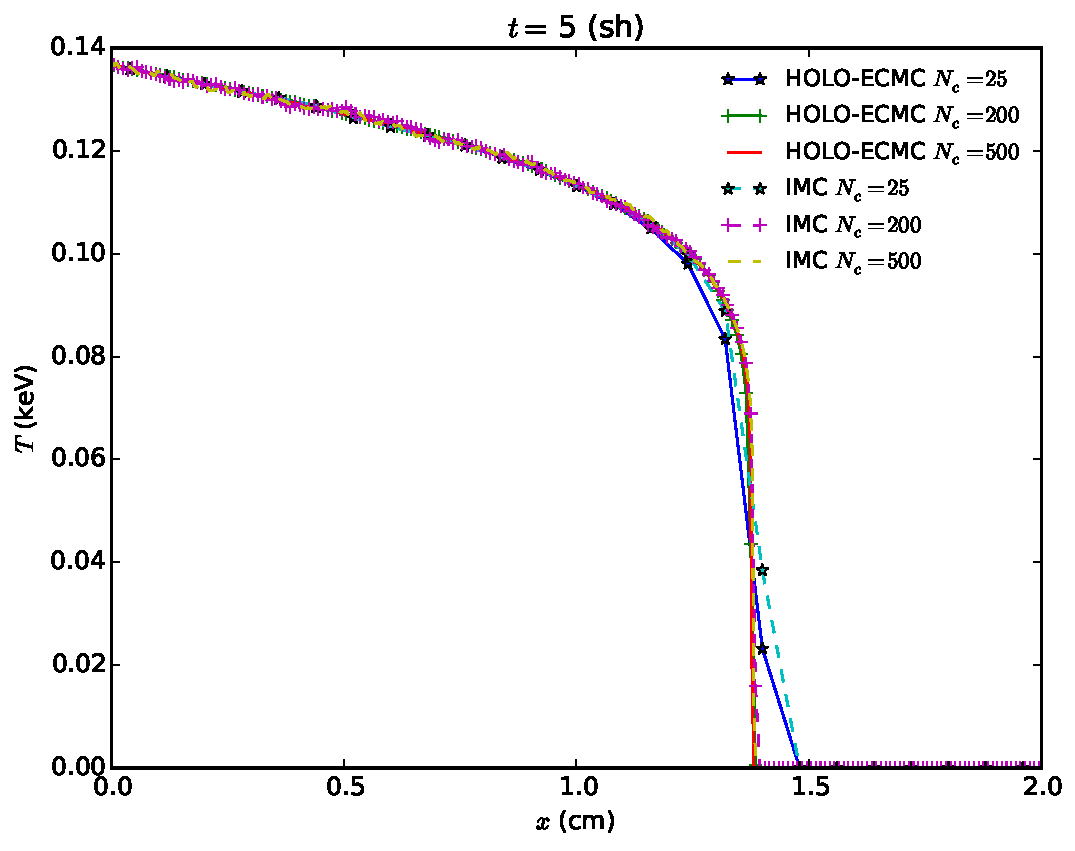
\includegraphics[width=0.99\linewidth]{marshak_mesh_conv.pdf}
    \caption{\label{marshak_mesh_conv} Spatial convergence of IMC and HOLO.}
\end{subfigure}
\begin{subfigure}{0.49\textwidth}
    \vspace{0.021in}
  \centering
  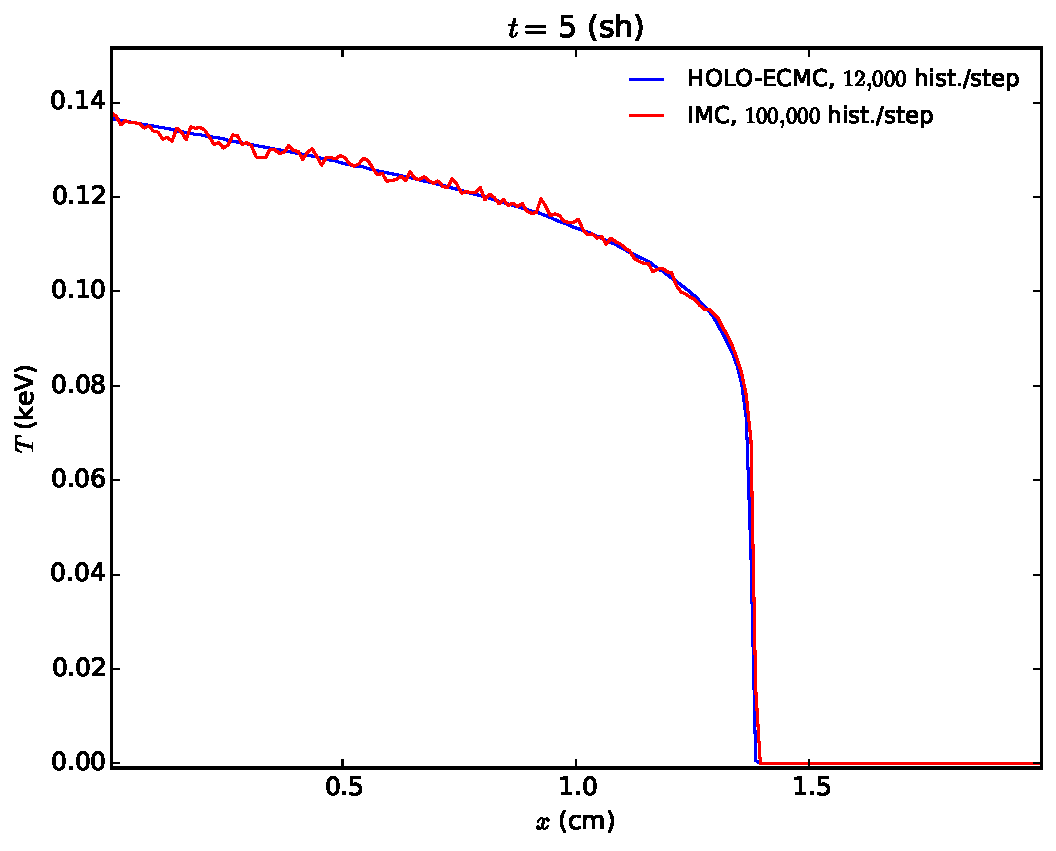
\includegraphics[width=0.99\linewidth]{marshak_200_compare.pdf}
  \caption{\label{marshak_200_compare}  Comparison of solutions for 200 spatial cells. }
\end{subfigure}
\caption{\bf Comparison of radiation temperatures for Marshak wave problem at $\mathbf{t=5}$ sh.}
\end{figure}

The second problem has similar behavior to the first problem, however the geometry consists of an optically thin (left) and an optically thick (right) material region,
with temperature-independent cross sections.  Fig.~\ref{twomat_full} compares the HOLO and IMC radiation 
temperatures at the end of the simulation. The
IMC and HOLO results show good agreement
over the finer mesh.
On the coarse mesh ($N_c=20$), the LDFE representation of $T^4$ in the HOLO method predicts the location of the
wave front more accurately than the source tilting of the IMC method.
Fig.~\ref{compare_ho} demonstrates the benefit of ECMC as a HO solver compared to
standard MC.  The HOLO algorithm
with the ECMC HO solver (HOLO-ECMC) results
are for running 3 batches of 10,000 histories, per time step. The solution for the HOLO method with a standard MC solver as the HO solver
(HOLO-SMC) with standard source sampling uses 10$^5$ histories per time step. The HOLO-SMC solution demonstrates significant
statistical noise.  This noise is introduced into the LO solver by poor statistics in
the MC computed consistency terms. Also
plotted is an S$_2$ solution obtained with consistency terms that are equivalent
to S$_2$ and no HO correction.  The S$_2$ solution results in an artificially fast
wave front, as expected, demonstrating the necessity of HO correction in this problem.
\begin{figure}[H]
    \centering
\begin{subfigure}{0.49\textwidth}
    \centering
    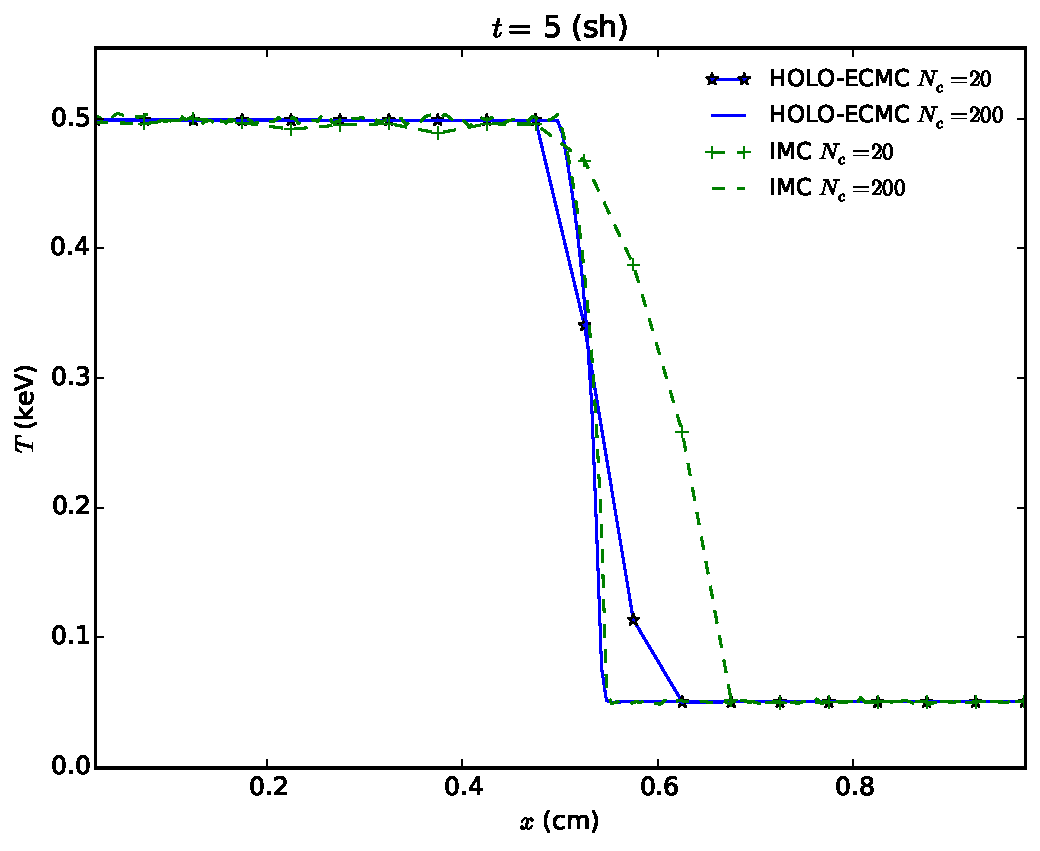
\includegraphics[width=0.99\textwidth]{two_mat_conv.pdf}
    \caption{Comparison of IMC and HOLO-ECMC.\label{twomat_full}}
\end{subfigure}    
\begin{subfigure}{0.49\textwidth}
    \vspace{0.16792in}
\centering
    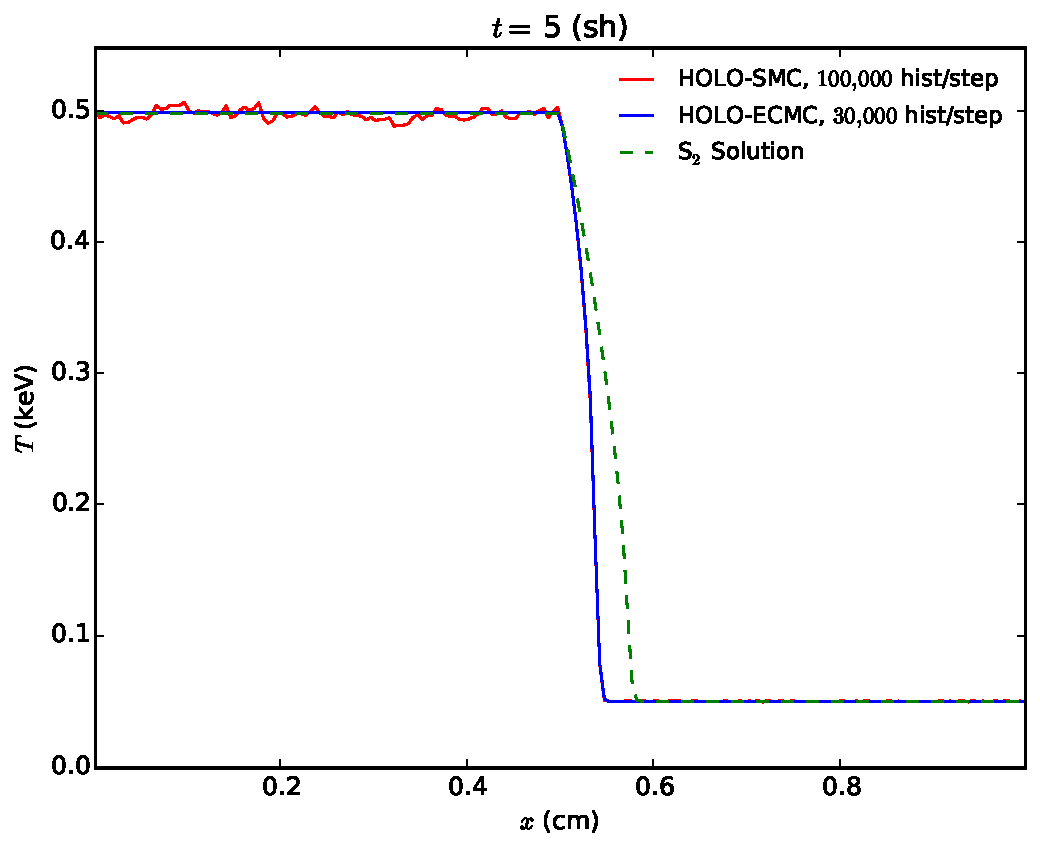
\includegraphics[width=0.99\textwidth]{two_mat_ho_compare.pdf}
    \caption{Comparison of SMC and ECMC HO solvers. \label{compare_ho}}
\end{subfigure}
    \caption{\bf Comparison of radiation temperatures for two material problem. \label{twomat}}
\end{figure}

\section{Discussion of Remaining Research}
\label{sec:prop}



\subsection{Resolving Issues in Optically Thick Cells}
\label{sec:negs}

The linear-discontinuous (LD) closure with upwinding is not strictly positive.  In particular, for
optically thick cells with a steep intensity gradient, the intensity becomes
negative. In typical TRT problems (e.g., the Marshak wave problems above), this negativity occurs at the wave-front of the
radiation intensity in optically thick materials.
These negativities are not physical and can propagate to adjacent cells. In thick regions of
TRT problems, reasonably fine spatial cells can still be on the order of millions of mean
free paths; negativities with an LD representation are unavoidable in practice for
such cells, and mesh refinement is of minimal use.  We will explore several methods
for resolving negativities.  Ideally the solutions in
such cells should be as consistent as possible for the HO and LO equations.  However,
the differences between the solution methods of the two equations, as well as the
fact that some terms are lagged, have lead to the development of independent
approaches for the LO and HO systems.

Typically, for a standard LDFE method,
the equations are lumped to produce a strictly positive solution (for 1D)~\cite{morel_newton}. However, standard FE lumping
procedures would introduce difficulties in computing the consistency terms from the
HO solution.  The lumping procedure does not guarantee positivity for the space-angle LDFE
representation of the HO intensity.  Additionally, the lumping approach is not
extendible to higher-dimensions where the choice of $S_2$ terms will not produce
accurate wave fronts for general problems.
Alternatively, the equations within a cell can be modified to ensure the outflow is not
below the floor value (the initial temperature of the problem), and energy balance is
conserved.  The LD shape is reconstructed by extrapolating from the outflow back
through the average.  This closure has been implemented and is more promising for extendability into higher
dimensions and for consistency with the HO approach.

For the HO solver, after an ECMC batch, we detect cells that produced a negative
intensity. In these cells, we scale the linear representation of the intensity (in
$x$ and $\mu$) to be greater than the floor
value.  This scaling process of the two moments is underdefined, so there is not a unique way to enforce
positivity.  The scaling procedure is not an emphasis of the research, so we apply the simple
approach of scaling the slopes such that the ratio of the slope in $x$ and $\mu$ is
unchanged.  The scaled intensity will not satisfy the original residual equation accurately because we have
modified the first moments.   Thus, the ECMC error estimates will rapidly stagnate,
and produce relatively inaccurate solutions.  This scaling can also lead to
negativities in down-stream cells that is unphysical in later batches.  To mitigate
stagnation and improve accuracy, we will add an artifical source $\tilde\delta^{m+1}(x,\mu)$ to the HO equation.
This source is estimated iteratively as
\begin{equation*}
    \tilde\delta(x,\mu)^{(m+1)} = \mathbf{L}(\tilde{I}^{n+1,(m)} -
    \tilde{I}^{n+1,(m)}_{\text{pos}}),
\end{equation*}
where $\tilde{I}_{pos}^{n+1}$ is the modified positive solution.
Essentially, this source is modifying the first moments of the transport equation to ensure a positive solution within the negative cells.  Neglecting
statistical noise, the solution will converge towards the strictly positive projection
$\tilde{I}_{\text{pos}}^{n+1}$ in the next batch. We can estimate the necessary source again in the next batch.  The source
$\tilde\delta$ lies in the same functional space as the residual, and thus can use
the existing code for computing the residual and will be straight forward to extend
to higher dimensions.  

We have implemented this artificial source and found it to reduce the
magnitude of the MC estimated error, producing a positive solution. We still need to
investigate the accuracy and robustness of the
added source method, and whether it should be recomputed every batch, once it has been
triggered, or only when the
solution becomes negative again.  Ideally, the added source will not alter the zeroth
moment of the solution, but that remains to be demonstrated numerically.  We will also
investigate adding the source to the LO equations for greater consistency and accuracy in
the LO equations.  This will not
necessarily guarantee positivity in the LO equations due to the fixed-point iteration
process.  We may need to alter the source computation to ensure that the zeroth moment
of the equations is not changed, ensuring energy conservation.

\subsection{Estimating the Spatial Closure from the HO Solution}

We will explore the possibility of a linear, doubly-discontinuous trial space in
in the HO and LO equations. This should allow for higher consistency between the HO and LO
equations. This trial space allows
the outflow from a cell to be discontinuous in space, introducing an extra
spatial unknown. This should produce greater
angular accuracy on faces in the HO solution.  In optically thick cells, this will mitigate observed issues with the spatial slope being
artificially high to account for the discrepancy in angular shape between the
internal and face solutions. A relation between the HO outflow and internal moments
will be used to eliminate the extra cell unknowns of the doubly-discontinuous trial
space in the LO equations, producing a consistent spatial closure between the HO and LO
solutions.  The linear shape on the interior of the cell is still necessary due to the
temperature unknowns.  In application, the HO outflow will be estimated using a
face-based tally of the MC solution.  It is possible that poor statistics in the face
tallies may result in this closure becoming inapplicable due to understampling in optically
thick regions.
It will also be necessary to ensure consistency with the LO
solution, particularly in the case of adaptively refined meshes and the
doubly-discontinuous trial space.  This will likely improve the accuracy in low-order
equations, but may not produce a more accurate solution in the HO equations.

\subsection{Diffusion Synthetic Acceleration of the LO Equations}

As described in Sec.~\ref{sec:lo_sol}, the fully-discretized LO equations can include
the scattering term in the system matrix.  This allows for the system to be directly
inverted.
However, an S$_2$ like system cannot be efficiently inverted
directly in higher spatial dimensions.  To demonstrate a possible path forward in
higher dimensions, we will investigate the use of a standard
source iteration scheme to solve the LO equations.  As
material properties become more diffusive (e.g., $c_v$ is small and $\sigma_a$ is
large), the effective scattering source becomes large.  This results in a spectral radius of the source iterations that approaches
unity~\cite{morel_newton}.  These regimes are typical in TRT simulations, so an
acceleration method is critical.  We will accelerate the source iterations with a nearly-consistent diffusion synthetic acceleration
(DSA) method~\cite{wla,wla_thesis}.

We can perform standard source iterations by lagging the scattering source in the LO
equations, which
uncouples unknowns between the two half-ranges.  This produces a lower-triangular
system where the spatial unknowns can be determined sequentially along the two directions of flow via a
standard sweeping procedure~\cite{lewis,morel_newton}.  The newly computed half-range
intensities can be used to compute the scattering source for the next iteration.  This
process is repeated until convergence.  
A form of DSA referred to as the WLA method is used to accelerate the source iterations~\cite{wla}. 
Between each source iteration, a residual equation is formed that provides 
the error in the current scattering iteration. The DSA method uses an approximate,
lower-order operator to estimate the error in the zeroth angular moment of the
intensity.  The DSA equations can be more efficiently
solved than the S$_2$-like sweeps that are being accelerated, but will accurately resolve the
slowly converging diffusive error modes.  It is important for the spatial discretization of the DSA
equations to be closely related to the discretization of the LO equations for the
acceleration to be effective.  The WLA method first solves a spatially-continuous
discretization of the diffusion equation
for the iterative error on faces.  The error on the faces is then mapped onto the
volumetric moment unknowns via a LD discretization of diffusion equation~\cite{wla}.
The LD mapping resolves issues that would occur in optically-thick cells, while the
continuous diffusion equation is accurate in the EDL where acceleration is important.

We have implemented the DSA algorithm and initial results indicate that the
acceleration is effective.  However, we have only considered the case when
the LO equations and DSA equations are lumped.  We will investigate the effect of acceleration when alternative negativity fix-ups are
implemented that result in DSA and LO equations that are not spatially consistent.
We will recast the DSA method as a preconditioner to an iterative
Krylov solution~\cite{larson_morel_sn} of the LO equations.  Generally, Krylov
methods mitigate acceleration losses due to inconsistencies in the acceleration
method.  In higher dimensions, the use of a Krylov method is necessary for effective
acceleration for nearly-consistent acceleration methods such as WLA in problems with
mixed optical thicknesses~\cite{larson_morel_sn}, e.g., typical radiative transfer
problems.
  We will apply the preconditioned-Krylov approach to allow for the use of lumped DSA
  equations as a preconditioner, with the LO equations using one of the other fixup
approaches detailed
in the previous section.  It is noted we are not interested in measuring the reduction of
computational time because in 1D the LO equations can be directly solved efficiently.
We are just interested in ensuring that DSA or a preconditioned-Krylov methods can reduce the
number of scattering iterations sufficiently, including cases where inconsistencies
in the LO equations are present.  %because DSA
%becomes less effective in mixed optical thicknesses and high spatial cell aspect
%ratios~\cite{morel_newton}.
%\subsection{Alternative time discretization}
%\label{sec:time}
%
%A final area of research to be investigated is in an alternative time discretization
%of the system.  This is the least developed portion of the research.  The goal of
%an alternative time discretization is to produce a more accurate solution in
%optically thin regions where particles transport a long distance.  This is an area
%where the MC treatment of the time-variable by IMC can produce greater accuracy,
%whereas a BE discretization will result in artificially fast propagation of energy.
%This may be important in applications such as stellar atmosphere calculations.  
%
%First, the ECMC
%solution is considered. The emission source
%is still treated as fully implicit, however the intensity is allowed to be continuous
%in time.  In inverting the $\B L$ operator, particles are born with some specific
%time, and their time is tracked until they reach the end of the time step.  Tallies are adjusted
%to account for the averaging over the time step.
%in terms of MC, letting . As with the spatial and angular variables, we assume a trial
%space for the time variable as well.  Two different options are considered.
%The first, is a doubly-discontinous treatement, where teh outflow in time is solved
%for with the MC.  Fig.~\ref{fig:dd_time} demonstrates the basic principle of this
%closure in time.  The second options is a linear discontinuous trial space in time.
%The first approach requires typical census type tallies~\cite{fig}, which adds
%significant complexity in terms of tallies.  The second will
%require the first moment in time to be tallied.  
%Again, ECMC will be computing the projection of the exact solution onto the trial
%space, so this will have the accuracy of IMC for the radiation.    Neither of these cases require the
%addition of Adds one extra set of unknowns to be stored. 
%
%Next, consistency with the LO system is
%necessary.  The goal is to not add additional equations to solve for the
%time-dependent unknowns, but to   Previous work has attempted to simply subtract the continuous HO solution
%from a BE discretziation of the discretized time-derivatives to add an artificial
%term, with the addition of extra terms from hydrodynamics~\cite{holo_rh}.  This has the added benefit that the LO solver exclusively deals in
%time-averaged unknowns.  As an alternative, we will estimate a parameter based on the
%ratio of the outflow in time to the average over the time step. One possible closure
%is
%\begin{equation}
%    I^{n+1} = 2\gamma_t \overline{I} - I^{n}
%\end{equation}
%where $\gamma_t$ is the closure factor and $\overline{I}$ is the time-averaged
%intensity.  A spatial and angle discretized version of the above equation can be used to
%eliminate the extra unknowns from the LO system.  The value of $\gamma_t$ is
%estimated by solving the above equation based on the latest HO solution for all
%parameters.  The stability and accuracy of these methods will need
%to be investigated. As a first step, a truly BE time discretization in the HO can be
%used in conjunction with the LO solver.





%
%  There
%is some difficulty in making the LO time-averaged quantities match with the HO
%solution, which may require some approximation.  However, this is not that different
%than the discrete case because the representation of $\tilde I^{n}$ is lagged an
%iteration anyways. 
%It is noted that the SIMC method explored 
%some similar alternate time discretizations for the temperature in the residual
%treatment, but second-order accurate time treatment.  However, the second-order approximation

\section{Summary and Outline of Remaining Research}
\label{sec:summary}

A new HOLO algorithm has been implemented, and results have demonstrated the ability
to reproduce IMC solutions accurately for two difficult Marshak
wave test problems.  The ECMC approach, with initial guesses based on the
previous radiation intensity, results in efficient reduction of statistical error and
allows for particles to be distributed to largely varying regions of the problem.
The LO solver resolves the non-linearities in the equations resulting in a fully
implicit time discretization. Overall, the LO solver 
can accurately and efficiently resolve the solution in diffusive regions, while the HO
transport solver provides the accuracy of a full transport treatment where necessary. 

We have proposed solutions to resolve issues in optically-thick cells and a source
iteration method for demonstrating the efficacy of our method.  The ability to overcome rapid stagnation in the ECMC algorithm when the solution cannot
be accurately represented by the trial space, e.g., negativities in optically thick
cells,  will be key for generalization of this
method to higher dimensions.  The goal of our proposed fixup is to mitigate the rapid
stagnation of ECMC iterations that would occur by forcing a positive solution each
batch.  Ideally, the added source will reduce the stagnation to order of the global
stagnation that occurs in other regions of the problem due to mesh resolution and a
finite number of histories per batch.  The LO and HO solutions will independently resolve issues with
negativities, with the goal of producing as consistent and accurate of solutions as
possible.  We also need to numerically demonstrate the
ability of DSA to accelerate our LO equations, in conjunction with a iterative Krylov
solution method.  There are other
desirable properties of our algorithm that remain to be tested, e.g., preservation of
the maximum principle.  In summary, we propose performing the following work to
complete this dissertation research:
\begin{enumerate}
    \item The source iteration method with DSA for the LO solver will be recast as a
        DSA-preconditioned Krylov method.  The scheme will be applied to test problems to ensure a significant reduction in total scattering
        iterations and the numerically estimated spectral radius in diffusive problems.  Problems that provide a mix of optically
        thick and thin regions, with the fix-ups defined in Sec.~\ref{sec:negs} will be investigated.
    \item Problems where IMC violates the maximum principle will be simulated with our
        method.  We will demonstrate that our implicit equations preserve the maximum
        principle, and that our method can produce higher accuracy due to implicit cross section
        treatment. Such problems will likely require implementation of damping in the
        Newton iterations.
    \item We will numerically demonstrate the ability of our method to preserve
        the equilibrium diffusion limit.  The HOLO method will also be tested with a step
        discretization in the LO equations to demonstrate inaccuracy in the EDL.
    \item The negativity fix-ups discussed in Sec.~\ref{sec:negs} will be investigated for robustness and
        accuracy.  The doubly-discontinuous fix-up with a consistent closure in the
        LO equations remains to be implemented.  An analytic neutronics problem or a refined deterministic TRT solution
        will be used to test for accuracy.  The ability of the modified ECMC
        algorithm to reduce noise in
        the fixup regions will be investigated by measuring sample statistics.
    \item We will investigate the sensitivity of ECMC and the LO equations to
        parameters, e.g., initial mesh-sizes, adaptive refinement, time step size, history
        counts, and batch sizes.  Additional test problems will be simulated as
        necessary.
\end{enumerate}
\pagebreak


\begin{spacing}{1}
  \bibliographystyle{unsrt}
  \bibliography{references}
\end{spacing}

\end{document}
